\subsubsection{QRCode I/O}
La gestione dei QRCode nel progetto è un aspetto molto importante, che coinvolge
e la fase di creazione di una cartà d'identità di un indivudio, e la fase di riconoscimento.
L'importanza dei QRCode risiede nel fatto che grazie ad essi, è possibile recuperare le features facciali ( firmate digitalmente ) per confrontarle con le features estratte al momento dell'identificazione.\\
Di consueguenza risulta essenziale generare un QRCode nella fase di creazione, e poter leggere il suo contenuto nella fase di autenticazione.
Per la gestione dei QRCode, è stata utilizzata una libreria OpenSource denominata 'ZXIng' \footnote{http://code.google.com/p/zxing/}, la quale permette di eseguire svariate operazioni con i codici a barre. Essendo la libreria Open, sono state estratte soltanto le funzionalità utili al progetto.
\paragraph{Generazione}
Per la generazione dei QRCode è stata realizzata una classe denominata "QRCodeEncoder" la quale offre dei metodi per generare un QRCode in formato "Bitmap", a partire da un insieme di dati quali dimensione del QRCode e i "byte" da inserire al suo interno. 
\begin{figure}[htbp]
   \centering
   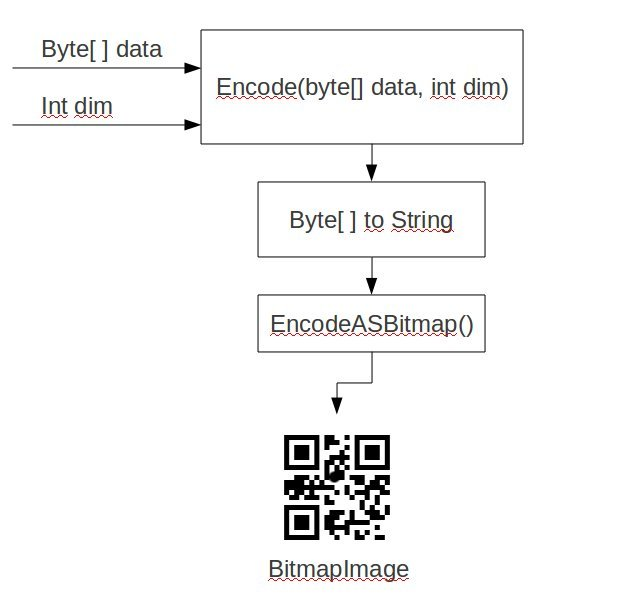
\includegraphics[width=6cm]{img/qrgen}
   \caption{Funzionamento della procedura di creazione del QRCode\label{qrgen}}
\end{figure}

Il vettore di byte passato alla funzione, viene convertito in un stringa, per poi essere codificato nel QRCode. In lettura si esegue il processo inverso.
La funzione dell'oggetto QRCodeEncoder è utilizzata staticamente nel progetto. Il metodo in questione è denominato \textit{encodeAsBitmap} ed esegue le operazioni appena descritte. Il metodo è utilizzato, richiamandolo staticamente in questo modo: \textit{QRCodeEncoder.encodeASBitmap(byte[] data, in dim)}.
Una volta che viene restituito l'oggetto Bitmap, questo verrà gestito dal programma, in modo tale da allegarlo alla mail che viene inoltrata all'amministratore del sistema.

\paragraph{Lettura}
La fase di decodifica deve essere effettuata per poter risalire alla features facciali appartenenti ad un indivuo.
La lettura di un QRCode è effettata grazie ad una scansione dalla videocamera di un dispositivo mobile.\\
Anche in questo caso, le librerie ZXIng offrono delle funzionalità per operare il processo di scansione.
A differenza della generazione, la lettura avviene lanciando una Intent esplicita in modalità: \textit{startActivityForResult}\footnote{Su Android è possibile invocare altre activity in varie modolità, tra le quali quella appena descritta. Le Activity lanciate in questo modo sono offrono un servizio, quindi per poter gestire il risultato deve essere implementato il metodo: OnActivityResult}.
La Intent viene dichiarata e lanciata in questo modo:
\begin{verbatim}
 Intent intent = new Intent("com.google.zxing.client.android.SCAN");
 intent.setPackage("com.google.zxing.client.android");
 intent.putExtra("SCAN_MODE", "QR_CODE_MODE");
 startActivityForResult(intent, 0);
\end{verbatim}
In lettura, viene implementato il metodo:
\begin{verbatim} 
public void onActivityResult(int requestCode, 
                             int resultCode, 
                             Intent intent)
\end{verbatim}, nel quale viene prelevato dalla intent, una stringa extra \begin{verbatim} intent.getStringExtra("SCAN_RESULT")
\end{verbatim}, la quale contiene il risultato della scansione.
Questo risultato sarà gestito in modo tale da ottenere il contenuto delle informazioni, ovvero le features facciali, firmate digitalemte.
\\
Il comportamento della lettura e della generazione dei QRCode è il seguente:
\begin{figure}[htbp]
   \centering
   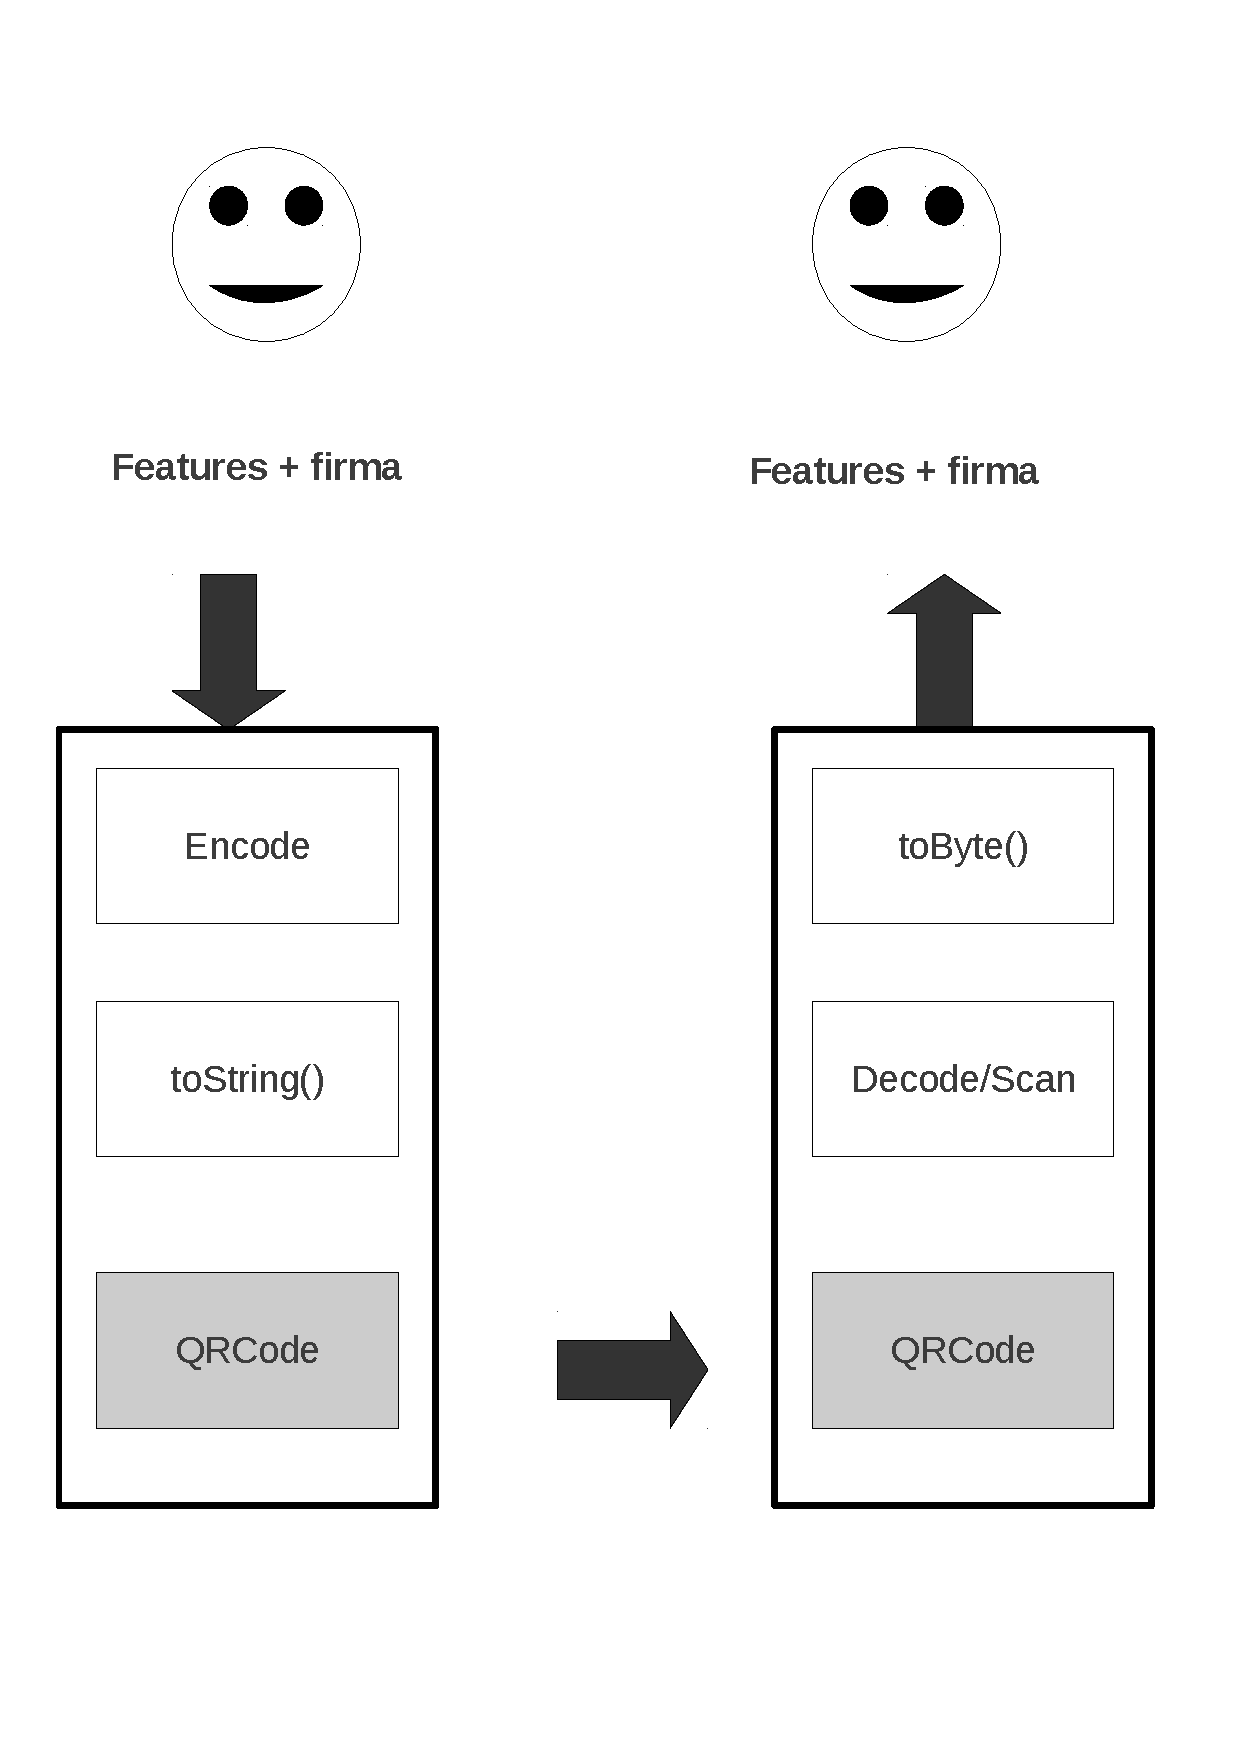
\includegraphics[width=6cm]{img/processo}
   \caption{Gestione QRCode fasi generazione - lettura\label{qrgen}}
\end{figure}